%%
%% StatisticalModel.tex
%% Login : <hoang-trong@hoang-trong-laptop>
%% Started on  Mon Jun 15 09:12:22 2009 Hoang-Trong Minh Tuan
%% $Id$
%% 
%% Copyright (C) 2009 Hoang-Trong Minh Tuan
%% This program is free software; you can redistribute it and/or modify
%% it under the terms of the GNU General Public License as published by
%% the Free Software Foundation; either version 2 of the License, or
%% (at your option) any later version.
%% 
%% This program is distributed in the hope that it will be useful,
%% but WITHOUT ANY WARRANTY; without even the implied warranty of
%% MERCHANTABILITY or FITNESS FOR A PARTICULAR PURPOSE.  See the
%% GNU General Public License for more details.
%% 
%% You should have received a copy of the GNU General Public License
%% along with this program; if not, write to the Free Software
%% Foundation, Inc., 59 Temple Place, Suite 330, Boston, MA 02111-1307 USA
%%

\chapter{Statistical models}
\label{chap:statistical-models}

A statitical model is a simplified description of data, usually
constructed from some mathematically or numerically defined
relationship.

Models are objects that imitate the properties of 'real' object, but in a
simpler and more convenient form. As the statistical model is never an exact
representation of the system, there is always a difference. The difference
between the model and 'reality' is called the {\it residuals}, and it is the key
for a deeper understanding the fitness of the model to the 'reality'.

Here are some examples of the models and the 'reality'.
\begin{itemize}
\item Architects use both paper drawing and small-scale physical
  models to imitate the properties of a building. Then, the appearance
  and other properties of the real house can be inferred from the
  model.

\item Chemists use wire-frame models of molecules (by constructing
  them or displaying them through computer graphics) to imitate the
  theoretical properties of the molecules that, in turn, can be used
  to predict the behavior of the real molecules.
\end{itemize}

A general criteria for a good model 'A good model reproduce as
{\bf accurate} as possible the relevant properties of the real object,
while being {\bf convenient} to use.' However, the collected data,
e.g. the test data in the fuel consumption example, does not cover all
the autombiles of interest; perhaps, we can use the model to mileage
of other automobiles. In other words, the goal is also to use the
model to understand or predict beyond the context of the current
data. For these reasons, useful statistical modeling cannot be
separated from questions of the design of the experiment, survey, or
other data-collection activity that produces the data.)
 
The choice of a statistical model depends on the application and on
the kinds of inference the users need to make. A general applied
criteria include simplicity; i.e. a model with fewer parameters or
explanatory variables.


\section{Creating a statistical model}
\label{sec:creat-stat-model}

Creating a statistical model is a multistage process.
\begin{enumerate}
\item Collecting data

\item Choose a candidate model (to describe some relation in the
  data) with some unknown free parameters

\item Fitting the model (usually by estimating some parameters based
  on some criteria, e.g. minimize least-quare error)

\item Summarizing the model to see what it say about the data

\item Using diagnostics (tables, verbal descriptions, and graphical
  displays) to see in what ways the model fail to fit as well as it
  should. Finally, decide whether another model should be chosen, or
  the model should be modified or it is good enough to describe the
  data.
\end{enumerate}

{\bf Example}: A formula to describe an additive model

\begin{verbatim}
        Mileage ~ Weight + Displacement
\end{verbatim}
which is interpreted as 'The Mileage consumption is modeled as Weight
plus Displacement' or the {\it response}, Mileage, can be predicted based
on the Weight of the car and the Number of miles, Displacement, the
car has been driven, as shown in Fig. \ref{fig:car_model}. These are
both linear model.

\begin{figure}[htb]
  \centerline{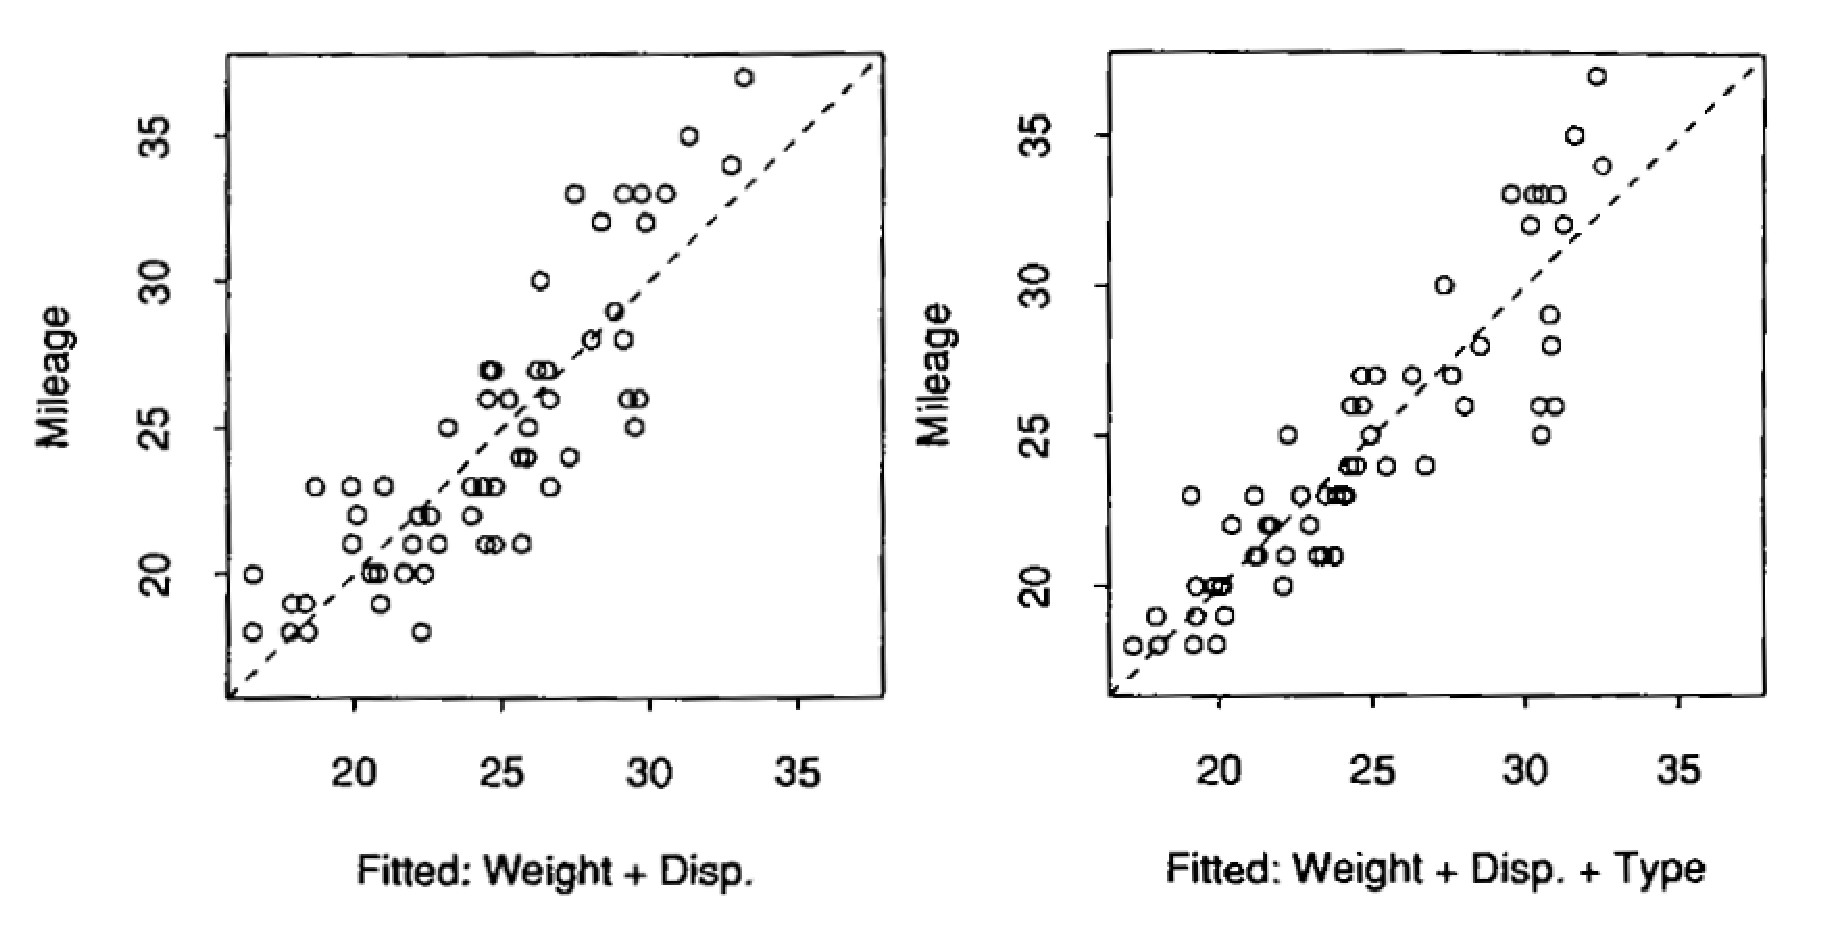
\includegraphics[height=6cm]{./images/sample_car_model.eps}}
  \caption{(a) Mileage \~ Weight + Disp; (b) Mileage \~ Weight +
    Disp + Type}\label{fig:car_model}
\end{figure}

If we plot the true value of Mileage and the values predicted by the
linear model in case (a), the model is not doing well for cars with
high mileage, i.e. they all fall above the line. However, if we add in
a coefficient for each type of car (compact, van, truck, sporty…) as
in case (b), the fit improves further. In practice, we would
continuously to study diagnostics and try alternative models, seeking
a better understanding of the underlying process.


To represent a model, R language use the concept of {\bf formula}.

\section{Error}
\label{sec:error}

Error is assumed to be normally distributed in most models

\section{A formula}
\label{sec:formula}

A statistical model tries to capture the relation, as a mathemtical function,
between the independent (explanatory) variables X1, X2, \ldots, Xn and the
response variable (dependent variable) Y: 
\begin{equation}
Y = f(X_1, X_2, \ldots, X_n)
\end{equation}
In order to produce the best models, {\bf regression analysis} is used and it
utilizes sample data (Sect.\ref{sec:regression_analysis}). 

\subsection{for a linear model}
\label{sec:linear-model}


A formula defines the structural part of a statistical model, i.e. the right
side after tilde (\textasciitilde). In order to define a formula, we need to
identify the {\bf response variable} and one or more {\bf predictor variables}.
Normally, we only have one response variable in a model, but there can be more
than one predictor.

{\bf A simple form of a formula is as follows}
\begin{verbatim}
         X ~ Y + Z
\end{verbatim}
where X is a response variable (or dependent variable); Y and Z are
two predictors (or independent variables).  This is the shorthand of
the predicting model, the '+' is not an algebraic addition, it is
being used in a special sense, to separate items in a list of terms to
be included in the model.


The form above is also similar to symbolic expression S or R. In S or
R, there is a type of object called {\bf formula} object which save
this structure. There is also a special function '\~"() that does
nothing but to save the formula as an unevaluated S expression, a
formula object.

Let's return to our basis example, the advantages of this
representation is that we don't need to specify the weighting
factors, in which the complete and correct representation should be
like this
\begin{equation}
  \label{eq:12}
  Mileage = \alpha + \beta_1 Weight + \beta_2 Disp + \varepsilon
\end{equation}
with $\varepsilon$ is the residual or the error side. There is no
information described here about how or what method should be used to
fit the model.

In R, we use the {\bf lm()} function for predicting the linear model
and the least square to compute the fitness.

\begin{lstlisting}
>> lm(Mileage ~ Weight + Fuel)
\end{lstlisting}
which is interpreted as 'Fuel is modeled as Power plus Weight' or
the response, Fuel, is represented by an additive model in two
predictors, Power and Weight.

The second point: the terms in a formula are not restricted to names
only (e.g. Weight, Fuel); they can be any S expression that, when
evaluated, can be interpreted as a variable.


{\bf Example}:If we want to model the logarithm of the Fuel, rather
than the Fuel itself
\begin{equation}
  \label{eq:17}
  \log(Fuel) \sim Power + Weight
\end{equation}

The third point: an independent variable in the formula may be a
\hyperref[sec:factor]{factor}, rather than a numeric. In the above
example, the car Type is a factor.

{\bf Example}: Consider this model where Salary and Age are numeric
vectors and Sex is a two-level factor
\begin{verbatim}
                  Salary ~ Age + Sex
\end{verbatim}
The complete representation should be as follows
\begin{equation*}
  \label{eq:18}
  Salary_i = \mu + \beta Age_i + \left\{ \begin{array}{rl}
     \alpha_M  & \text{if } Sex_i \text{ is male} \\
     \alpha_F & \text{if } Sex_i \text{ is female} \\
\end{array} \right. + \varepsilon_i
\end{equation*}
So, the two numeric values $\alpha_M, \alpha_F$ represent two levels
of Sex parameter.  This model can be represented by an equivalent one
if we create two dummy variables Xmale and Xfemale in which Xmale is
set to 1 for all male observations and 0 otherwise and Xfemale is set
to 1 for all female observations and 0 otherwise.
\begin{verbatim}
                  Salary ~ Age + Xmale + Xfemale
\end{verbatim}
Other non-numeric variables enter a model by being interpereted as
factors. Example:
\begin{itemize}
\item A logical variable is interpreted as a factor with two
  levels 'TRUE' and 'FALSE'.

\item A character variable is interpreted as a factor with levels
  equal to the set of distinct character strings

\item A category object in S or R will be treated as a factor in
  modeling software
\end{itemize}

The fourth point: a term in a formula can also refer to a
matrix. Then, each column of the matrix will appear linearly in the
model with its own coefficient. However, the entire matrix is
still interpreted as a single term.

In summary: the following S or R data types can appear in a formula
\begin{itemize}
\item a numeric vector, implying a single coefficient

\item a factor or an ordered factor, implying one coefficient for each
  level

\item a matrix, implying a coefficient for each column

\item any S expression whose evaluated results corresponding to one of
  the three types above, for example
  \begin{itemize}
  \item $(Age > 40)$
  \item cut(Age,3)
  \item poly(Age,3)
  \end{itemize}
\end{itemize}


Here are some examples of more complicated formula
\begin{itemize}
\item This is a little bit complicated formula
\begin{verbatim}
            100/Mileage ~ poly(Weight, 3) + sqrt(Power)
\end{verbatim}
  means the model needs to fit the derived variable, 100/Mileage, to a
  third-order polynomial in Weight plus the square-root of the Power
  variable.

\item A formula to fit the B-spline regression curves within two
  levels of Power obtained by cutting Power at its mid-range
\begin{verbatim}
Fuel ~ cut(Power, 2) / bs(Weight, df = 5)
\end{verbatim}

\item A nonparametric smooth curve will be used to model the
  transformed Fuel additively in Weight and Power, using 5 degrees of
  freedom for each term
\begin{verbatim}
sqrt(Fuel-min(Fuel)) ~ s(Weight, df = 5) 
                      + s(Power, df = 5)
\end{verbatim}
\end{itemize}


\subsection{for a non-linear model}
\label{sec:non-linear-model}

For nonlinear model, the formula will have to be completely explicit,
i.e. we need to specify the weighting factors. Besides, we noted that
the formula make no reference to the error $\varepsilon$ either. This
is the stochastic part of the model specification.

\section{The stochastic part of the model}
\label{sec:stoch-part-model}




%%% Local Variables: 
%%% mode: latex
%%% TeX-master: "R_language"
%%% End: 
\section{Regression analysis}
\label{sec:regression_analysis}

Regression analysis is used when the response variables and the explanatory
variables are {\it continuous}. For discrete outcome, we use {\it
classification} or {\it pattern-recognition} techniques.


The simplest and most common form is {\bf linear regression}. The goal is to
minimize loss (Sect.\ref{sec:linear_regression}) or minimize transformed loss
(Sect.\ref{sec:generalized_linear_regression}).

In the case of logistic regression (Sect.\ref{sec:logistic_regression}), it
applies to categorical (discrete) outcome by maximizing the likelihood.

An important notice is that {\bf homoscedasticity} is VERY important in the
application of regression analysis, including analysis of
variances.\footnote{\url{http://en.wikipedia.org/wiki/Heteroscedasticity}} To
test if the data is heteroscedasticity, read Chap.\ref{chap:heteroscedasticity}.

\subsection{Linear regression}
\label{sec:linear_regression}

{\bf Linear regression} is a regression analysis
(Sect.\ref{sec:regression_analysis}) technique in that the outcome (e.g.
the housing price) is a continuous-valued quantity, and is expected to be a
linear function of the input variable.

It's all about 'learning' some functional form. Suppose 
\begin{equation}
\mathbf{y} = h_\theta(\mathbf{x}) = \theta^T \mathbf{x}
\end{equation}
As a linear function, it can be represented in the matrix-vector operation.
We need to estimate the parameters (coefficients) in the transposed matrix
$\theta^T$.

\begin{mdframed}
NOTE: With $\mathbf(x) = (x_1, x_2)$, then
\begin{equation}
\mathbf{y} = h_\theta(\mathbf{x}) = \theta_0 + \theta_1 x_1 + \theta_2 x_2 = 
  \sum_{i=0}^n \theta_i x_i = \theta^T \mathbf{x}
\end{equation}
The $\theta_i$'s are the parameters
(also called weights) parameterizing the
space of linear functions.

\end{mdframed}

Example of {\bf linear regression}:
we want to predict the continuous-valued quantities (e.g., housing prices) as a
linear function of input values (e.g., the size of the house).

Here $y$ is the housing-price, and $x$ is the information about size of the
house
\begin{equation}
\begin{split}
\hat{y} &= a + b \times \mathbf{x} \\
\text{or} \\
\hat{y} &= a + b_1 \times x_1 + b_2 \times x_2 + \ldots b_n \times x_n
\end{split}
\end{equation}
with $y$ is the response variable, and $\mathbf{x}$ is the explanatory
variable which can be vectors. The two important factors: \verb!a! and \verb!b! are the
intercept and slope, respectively, in the $n$-dimensional space. The third
important factor is the correlation \verb!r!.

\begin{framed}
The validation of the linear model depends on the following assumptions of the
residual $r = (y-\hat{y})$
\begin{enumerate}
  \item Homoscedasticity (constant variance), i.e. the variance of $r$ is
  constant across the indices or the point should be evenly distributed around
  the mean. To test, we can plot $r$ vs. $y$, which if shows a dependence
  pattern then the linear model is likely INVALID. To overcome this, i.e. try to
  map to a linear model, then we can use data $\log(y)$, rather than $y$, or use
  a more complicated explanatory variables, e.g. $x_1^2$ or $x_1x_2$.
   
  \item Normality of errors, i.e. $r$ is normally distributed. Thus, RSS
  satisties $\chi^2$-distribution. The smaller RSS, the better the estimated
  model.
\end{enumerate}
\end{framed}

\subsection{-- cost function}

Now, giving the training data set
\begin{verbatim}
Living area (feet^2)   #bedrooms    Price (1000$s)
2104                   3            400
1600                   3            330
2400                   3            369
1416                   2            232
3000                   4            540
...                   ...             ...
\end{verbatim}
The question is how can we estimate the parameters $\theta$.

One reasonable method seems to be to make $h_\theta(\mathbf{x})$ close to y, we
can define the {\bf cost function} using using Least-Square Fit (i.e. minimum
square loss model)
\begin{equation}
\begin{split}
J(\theta) = \frac{1}{2} \sum_{i=1}^m \left( h_\theta(\mathbf{x}^{(i)}) -
y^{(i)}\right)^2  \\
= \sum^n_{i=1} \left( \hat{y}^{(i)} - y^{(i)}\right)^2
\end{split}
\end{equation}
%= \sum^n_{i=1} \left(y_i - \hat{y}_i \right)^2


i.e. find \verb!a! and \verb!b! to minimize the value of RSS $J(\theta)$. This
is simple Calculus I problem  with a unique minimum and unique pair (a,b) to
achieve this.
For a model with multiple input, i.e. \verb!x! is a vector like the second form
given above, this is called multiple linear regression. We still have a unique
solution, yet we now need to solve matrix algebra rather than simple algebra.

\subsection{-- R code  (R: lm function)}

\textcolor{red}{In R language}:
\begin{verbatim}
// to build the linear model
// lmFit <- lm( Y ~ X1 + ... + Xk)
// NOTE: We don't use ... but put as many Xk we want there


> lmFit <- lm( Y ~ X1 + X2 + X3 + X4)
\end{verbatim}
NOTE: We don't need to write the coefficients here. The statistics measuring the
goodness of fit and estimated coefficients of the model is given by calling
\begin{verbatim}
> summary(lmFit)

// Example output
Residuals:
Min 1Q Median 3Q Max
-1.176 -0.403 -0.106 0.524 1.154
Coefficients:
Estimate Std. Error t value Pr(>|t|)
(Intercept) 4.660 1.098 4.24 0.00082
x1 3.235 1.207 2.68 0.01792
x2 3.147 0.688 4.57 0.00043
x3 -6.486 1.881 -3.45 0.00391
x4 -1.117 0.596 -1.87 0.08223
x5 1.931 0.241 8.03 1.3e-06

Residual standard error: 0.684 on 14 degrees of freedom
Multiple R-Squared: 0.974, Adjusted R-squared: 0.965
F-statistic: 106 on 5 and 14 DF, p-value: 1.30e-10
\end{verbatim}

We can extract $\hat{y}$ vectors, i.e. of fitted values
\begin{verbatim}
> lmFit$fitted.values

> names(lmFit)   // display other names we can use
          // like fitted.values
\end{verbatim}

\subsection{-- Interview question}

In the linear regression model, the slope of the linear line is expected to be
fixed. However, in many applications, the model should be fitted by multiple
linear models, each associated with a given segment/range of data.

{\bf Interview Question}: How to modify a linear regression model to deal with
data which are linear, however the slope is time changing (for example, you can
divide the data into several segments in time, at each segment, the slope would
be found to be different), and most possibly, the slope follows a continuous
distribution, like Gaussian, for example


\subsection{Generalized Linear regression (R: glm function)}
\label{sec:generalized_linear_regression}

By transforming a variable or including interactions between the variables, we
can have more complicated linear regression models
\begin{verbatim}

log(y) ~ a + c_1 x_1 + c_2 x_1^2 + c_3 x_2 + c4 x_1 x_2
\end{verbatim}
The model is still linear as it is linear in the parameters. R language can
handle this using {\bf glm}.

\begin{framed}
For predicting a categorical outcome (such as y = true/false) it is often
advised to use a form of GLM called a {\bf logistic regression} instead of a
standard linear regression. 
\end{framed}

Example data:
\begin{verbatim}
> d <- read.table(file='http://www.win-vector.com/dfiles/glmLoss/dGLMdat.csv',
    header=T,sep=',')
> d
            x1          x2     y
1   0.09793624 -0.50020073 FALSE
2  -0.54933361  0.00834841  TRUE
3   0.18499020 -0.79325364  TRUE
4   0.58316450  2.06501637  TRUE
5   0.09607855  0.42724062  TRUE
6  -0.44772937  0.23267758 FALSE
7   1.24981165 -0.24492799  TRUE
8   0.13378532 -0.21985529  TRUE
9   0.41987141 -0.63677825 FALSE
10  1.28558918  1.37708143 FALSE
11  0.32590303  0.90813181  TRUE
12  0.01148262 -1.35426485 FALSE
13 -0.98502686  1.85317024  TRUE
14 -0.23017795 -0.06923035 FALSE
15  1.29606888 -0.80930538  TRUE
16  0.31286797  0.21319610  TRUE
17  0.03766960 -1.13314348  TRUE
18  0.03662855  0.67440240 FALSE
19  1.62032558 -0.57165979  TRUE
20 -0.63236983 -0.30736577 FALSE
\end{verbatim}

\subsection{-- Logistic regression (y=true/false)}
\label{sec:logistic_regression}

\begin{mdframed}
Example data: above \verb!y! get either true or false, which if we use a regular
linear model
\begin{verbatim}
lm(y ~ x1 + x2, data=d)
\end{verbatim}
then (behind the scences) R encodes y=true as 1 and y=false as 0 (R's default
encoded approach as an indicator). The result of fitting the model to a
categorical outcome is overly dependent on how you encoded the data as an
indicator. An example here is if the predicted value is '2', it still get the
same penalty as returning the predicted value to '0', if the true value is '1'. 
It means that the model can be penalized for being 'too right'. The solution is
to use {\bf logistic regression}, which is also a form of Generalized linear
regression (Sect.\ref{sec:generalized_linear_regression}).

\end{mdframed}

{\bf Logistic regression} is one regression analysis technique
(Sect.\ref{sec:regression_analysis}), yet it can be considered as a simple
classification problem (Sect.\ref{sec:classification}), in that we  wish to
predict a discrete variable such as predicting whether a grid of pixel
intensities represents a '0' digit or a '1' digit.

It's all about 'learning' some functional form. 
With logistic regression, i.e. two-class, we try to learn the 'sigmoid' or
logistic fuunctional form which is an S-shaped function that squash the value of
$\theta^T x	$ into the range [0,1] so that we may interpret the value of
$h_\theta(x)$ as a probability.

\begin{equation}
\begin{split}
P(y=1 | x) = h_\theta(x) = \frac{1}{1+\exp\left( -\theta^T x \right)} =
\sigma(\theta^T x) \\
P(y=0 | x) = 1 - P(y=1 | x) = 1 - h_\theta(x)
\end{split}
\end{equation}



To constrain the output always in the range [0,1], we use the sigmoid function
\begin{equation}
s(z) = \frac{1}{1+e^{-z}}
\end{equation}
The sigmoid s() has the following properties:
\begin{enumerate}
  \item s($-\infty$) = 0
  \item s($\infty$) = 1
  \item s(0) = 1/2
  \item s(-x) = 1 - s(x)
  \item x > y implies s(x) >  s(y)
  \item s'(x) = s(x)(1-s(x))
\end{enumerate}

And the new linear regression model (i.e. {\it logistic regression model}) is 
\begin{verbatim}
y = s * (a + b*x1 + c*x2) 
\end{verbatim}
Here, using the above data, the model supplies probabilities for each datum and
the 
\begin{verbatim}
m <- glm(y~x1+x2,data=d,family=binomial(link='logit'))
summary(m)
\end{verbatim}

To produce the model that is most consistent with the model, what it does is to
fit the maximum likelihood to the data, i.e. the model tends to yield  high
values on y=true samples, and otherwise. The {\bf maximum likelihood} solution
picks the coefficients $a,b,c$ to maximize
\begin{equation}
\left( \Pi_{i:y_u=\text{TRUE}} s(a+bx_{1i} + cx_{2i})\right)
\left( \Pi_{i:y_u=\text{FALSE}} s(a+bx_{1i} + cx_{2i})\right)
\end{equation}
NOTE: This is not the same as minimizing RSS in linear regression,
which is 
\begin{equation}
\sum_i \left( s \times (a+bx_{1i}+cx_{2i}) -\delta_{y=\text{TRUE}} \right)^2
\end{equation}

\url{http://www.r-bloggers.com/what-does-a-generalized-linear-model-do/}

\subsection{Lasso-based regression}
\label{sec:Lasso-regression}




\section{Fitting a linear model}
\label{sec:fitting-linear-model}


Fitting a linear model can be done easily in R statistics with {\bf
  lm(formula, data)} function (Sect.\ref{sec:linear_regression}) or {\bf
  glm(formula, data)} (Sect.\ref{sec:generalized_linear_regression}).

\begin{lstlisting}
> g = read.csv('galton-heights.csv')
 family father mother sex height nkids
1   1    78.5    67.0  M   73.2   4
2   1    78.5    67.0  F   69.0   4 
...
6   2    75.5    66.5  M   72.5   4

> lm( height ~ sex + father, data=g)
(Intercept) sexM father
34.4611 5.1760 0.4278

> lm( height ~ sex + father + mother, data=g)
(Intercept) sexM father mother
15.3448 5.2260 0.4060 0.3215
\end{lstlisting}

\begin{lstlisting}
> sum( g$height^2)
[1] 4013892> m1 = lm( height ~ sex + father, data=g)

> sum( m1$fitted^2) + sum( m1$resid^2)
[1] 4013892

> m2 = lm( height ~ sex + father + mother, data=g)

> sum( m2$fitted^2) + sum( m2$resid^2)
[1] 4013892
\end{lstlisting}

Orthogonality of fitted and residual
\begin{lstlisting}
> sum( m2$fitted * m2$resid )
[1] 4.239498e-12 -- essentially 0
\end{lstlisting}

Summary
\begin{lstlisting}
> m3 = lm( height ~ sex + father + mother + nkids, 
            data=g)
> summary(m3)
           Estimate Std. Error t value Pr(>|t|)
(Intercept) 16.18771 2.79387 5.794 9.52e-09
sexM        5.20995 0.14422 36.125 < 2e-16
father      0.39831 0.02957 13.472 < 2e-16
mother      0.32096 0.03126 10.269 < 2e-16
nkids      -0.04382 0.02718 -1.612 0.107

> anova(m3)
           Df Sum Sq Mean Sq F value Pr(>F)
(Intercept) 1 4002377 4002377 8.6392e+05 <2e-16
sex         1 5875 5875 1.2680e+03 <2e-16
father      1 1001 1001 2.1609e+02 <2e-16
mother      1 490 490 1.0581e+02 <2e-16
nkids       1 12 12 2.5992e+00 0.1073
Residuals 893 4137 5
\end{lstlisting}


\section{Bootstrap statistics}

%TODO: write bootstrap statistics


\section{Circular statistics}

